%! suppress = NonBreakingSpace
\documentclass[a4paper,12pt]{article}
\usepackage[english, finnish]{babel}
\usepackage{setspace}
\usepackage{makecell}
\usepackage{layout}
\usepackage{graphicx}
\usepackage{geometry}
\usepackage{lastpage}
\usepackage{listings}
\usepackage{multirow}
\usepackage{amsmath}
\usepackage{url}
\usepackage{listings}
\usepackage{listings-rust}
\usepackage{tikz}
\usepackage{setspace}
\usepackage{framed}
\usepackage{parskip}
\usepackage[style=vancouver]{biblatex}
\usepackage{xcolor}
\usepackage{tabularray}
\usepackage{tabularx}
\usepackage[T1]{fontenc}
\usepackage{csquotes}

%\usepackage{helvet}
%\renewcommand{\familydefault}{\sfdefault}
\usepackage{fontspec}
\setmainfont{Arial}


\addbibresource{mendeley.bib}
% \usepackage{showframe}
\lstset{language=Rust, style=boxed,
    captionpos=b,
    literate={ö}{{\"o}}1
        {ä}{{\"a}}1
}
\renewcommand{\lstlistingname}{Lähdekoodi}
\interfootnotelinepenalty=10000

\definecolor{title}{RGB}{155, 50, 35}


\usepackage{tikz}
\usetikzlibrary{positioning,shapes,shadows,arrows}

\tikzstyle{struct}=[rectangle, draw=black, text centered, anchor=north, text=black, text width=4cm]
\tikzstyle{thread}=[rectangle, draw=black, text centered, anchor=north, text=black, text width=4cm]
\tikzstyle{app}=[rectangle, draw=black, text centered, anchor=north, text=black, text width=3cm]



\newcommand{\architecture}{
\begin{figure}[h!]
\centering
    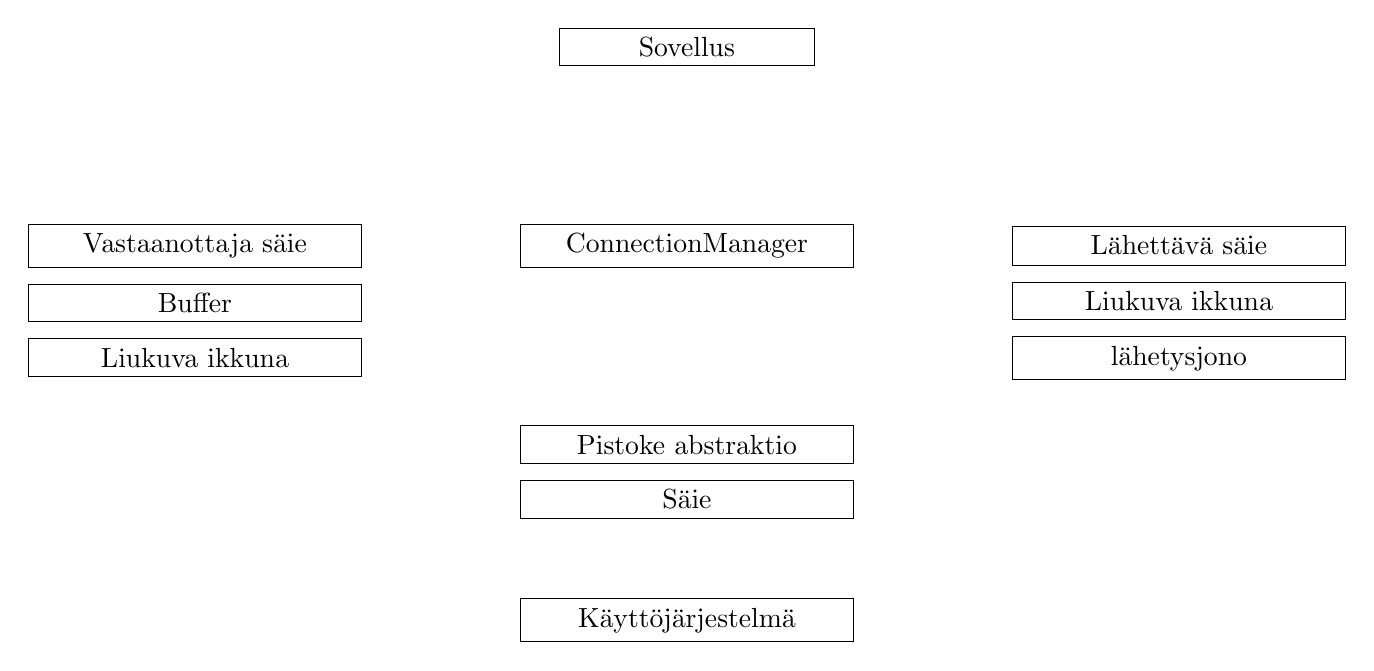
\begin{tikzpicture}[node distance=2cm]
        \node(app)[app]{
            Sovellus
        };
        \node(ConnectionManager)[struct, below=of app] {
            ConnectionManager
        };
       \node(rthread)[thread, left=of ConnectionManager]{
            Vastaanottaja säie
       };
       \node(buffer)[struct, below=0.2cm of rthread] {
            Buffer 
       };
       \node(rwindow)[struct, below=0.2cm of buffer] {
            Liukuva ikkuna 
       };
       \node(tthread)[thread, right=of ConnectionManager]{
            Lähettävä säie
       };
       \node(twindow)[struct, below=0.2cm of tthread] {
            Liukuva ikkuna 
       };
       \node(queue)[struct, below=0.2cm of twindow] {
            lähetysjono
       };
       \node(socket)[struct, below=of ConnectionManager]{
            Pistoke abstraktio
       };
       \node(socketthread)[struct, below=0.2cm of socket]{
            Säie
       };
       \node(os)[struct, below=1cm of socketthread]{
            Käyttöjärjestelmä
       };
    \end{tikzpicture}
    \caption{Arkkitehtuuridiagrammi} \label{fig:arkkitehtuuri}
\end{figure}
}
\usepackage{tikz}
\usetikzlibrary{positioning,shapes,shadows,arrows,quotes,fit}

\tikzstyle{data}=[rectangle, draw=black, text centered, anchor=north, text=black, inner sep=0.5cm]

\tikzstyle{title}=[font=\fontsize{6}{6}\color{black!50}]

\usetikzlibrary{arrows.meta}
\tikzset{>={Latex[scale=1.2]}} 


\newcommand{\slidingWindow}{
\begin{figure}[h!]
\centering
    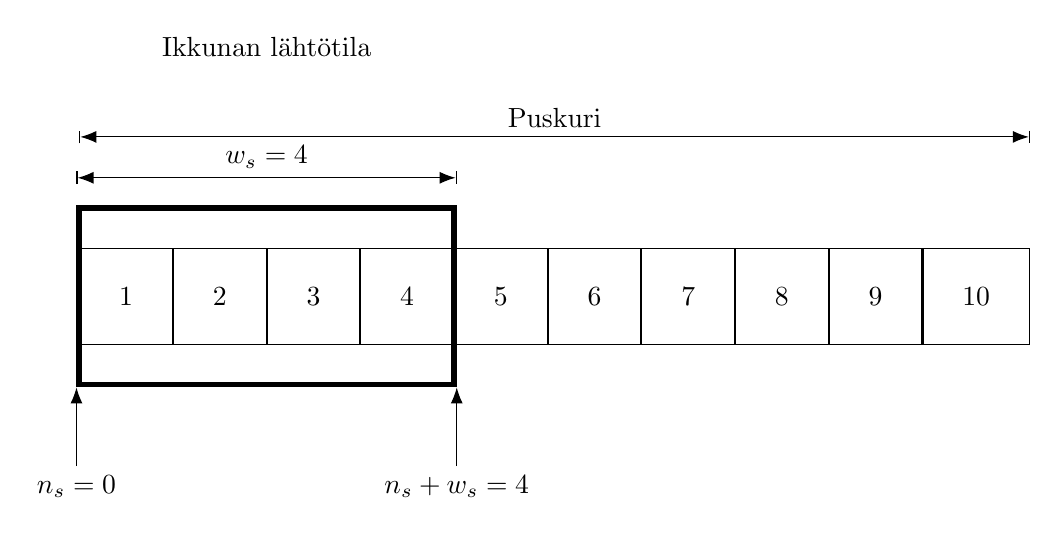
\begin{tikzpicture}[]
        
        \node(data1)[data]{1};
        \foreach \x [remember=\x as \lastx (initially 1)] in {2,...,10}{
            \node(data\x)[data, right=0cm of data\lastx]{\x};
        };
        
        
        \node (window) [draw=black, line width=2pt, inner xsep=0, inner ysep=0.5cm, fit=(data1) (data2) (data3) (data4) ] {};
        
        \node (windowStart)[below=of window.south west]{$n_s = 0$};
        \draw [->] (windowStart) -- (window.south west);
        
        \node (windowEnd)[below=of window.south east]{$n_s + w_s = 4$};
        \draw [->] (windowEnd) -- (window.south east);
        
        \node (windowDesc) [above=5.0em of window] {Ikkunan lähtötila};

        \draw [|<->|] ([yshift=1em]window.north west) -- node[above] {$w_s = 4$} ([yshift=1em]window.north east);
       
        \draw [|<->|] ([yshift=4.0em]data1.north west) -- node[above] {Puskuri} ([yshift=4.0em]data10.north east);
        
    \end{tikzpicture}
    \\[1cm]
    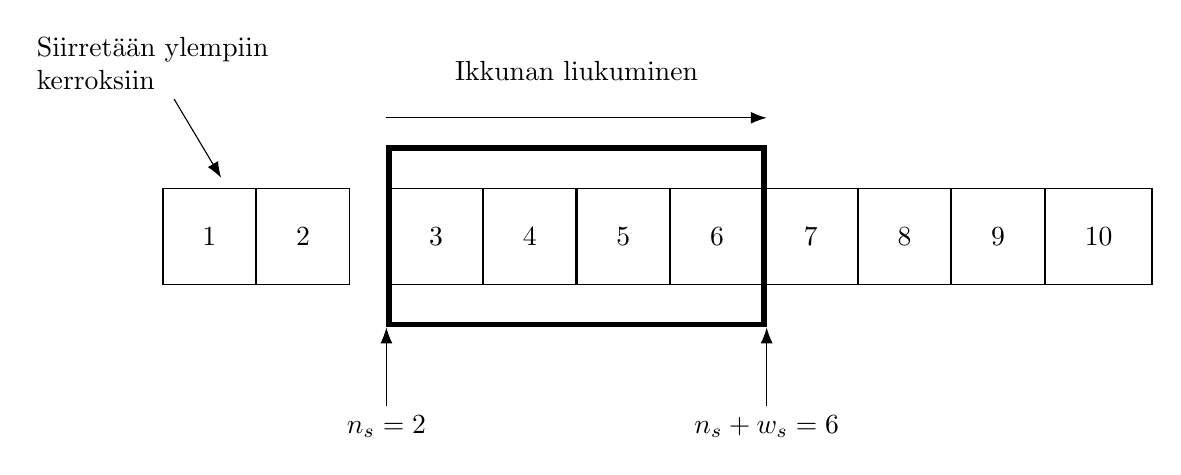
\begin{tikzpicture}[]
    
        \node(data1)[data]{1};
        \node(data2)[data, right=0cm of data1]{2};
        \node(data3)[data, right=0.5cm of data2]{3};
        \foreach \x [remember=\x as \lastx (initially 3)] in {4,...,10}{
            \node(data\x)[data, right=0cm of data\lastx]{\x};
        };

        \node (shiftedNodes) [fit=(data1) (data2)] {};

        \node (shiftDesc) [above=of shiftedNodes.north west, align=left] {Siirretään ylempiin \\kerroksiin};
       \draw [->] (shiftDesc) -- (shiftedNodes) {}; 
        
        \node (window) [draw=black, line width=2pt, inner xsep=0, inner ysep=0.5cm, fit=(data3) (data4) (data5) (data6) ] {};
        
        
        \node (windowDesc) [above=2.0em of window] {Ikkunan liukuminen};

        \node (windowStart)[below=of window.south west]{$n_s = 2$};
        \draw [->] (windowStart) -- (window.south west);
        
        \node (windowEnd)[below=of window.south east]{$n_s + w_s = 6$};
        \draw [->] (windowEnd) -- (window.south east);
        
        \draw [->] ([yshift=1em]window.north west) -- ([yshift=1em]window.north east);
        
    \end{tikzpicture}
    \caption{Liukuvan ikkunan toiminta} \label{fig:sliding_window}
\end{figure}
}


\onehalfspacing


\usepackage{hyperref}
\hypersetup{
    colorlinks,
    citecolor=black,
    filecolor=black,
    linkcolor=black,
    urlcolor=black
}



\renewcommand{\title}{Tietoliikenneprotokollan kehitys UDP:n päälle}
\newcommand{\englishTitle}{Development of transport protocol on top of UDP}

\author{Joonas Kajava}
\date{\today}

\newcommand{\me}{Joonas Kajava}

\newcommand{\appendixCount}{0}

\newcommand{\pageCount}{ \pageref{LastPage}}

\newcommand*\sepline{
    \begin{center}
        \rule[1ex]{\textwidth}{.5pt}
    \end{center}}


\begin{document}
    \begin{titlepage}
    
        \pagestyle{empty}
        
        
\includegraphics[width=0.5\textwidth]{images/metropolia}\par\vspace{2cm}
        {\Large \me}\par \vspace{1cm}

        {\Huge \textcolor{title}{\title}}\par \vspace{1cm}

        \vfill

        Metropolia Ammattikorkeakoulu\par
        Insinööri (AMK)\par
        Tieto ja viestintätekniikka\par
        Insinöörityö\par
        \today

        \newpage



        \section*{Tiivistelmä}

        \begin{tabular} {l l}
            Tekijä:               & \me                                            \\
            Otsikko:              & \title                                         \\
            Sivumäärä:            & \pageCount{} sivua + \appendixCount{} liitettä \\
            Aika:                 & \today                                         \\
            \\
            Tutkinto: & Insinööri (AMK) \\
            Tutkinto-ohjelma: & Tieto- ja viestintätekniikka \\
            Ammatillinen pääaine: & Pelisovellukset \\
            Ohjaajat: & Lehtori Miikka Mäki-Uuro\\
        \end{tabular}
        \sepline
        \begin{singlespace}
        
        Tämä insinöörityö käy läpi tietoliikenneprotokollan kehityksen UDP:n päälle. Protokollaa varten tehtiin ohjelmakirjasto Rust-kielelle, minkä toteutus ja toiminta käydään työssä läpi. Lopputuloksena syntyi RRTP-protokollan toteuttava ohjelmakirjasto, joka yhdistää liukuvan ikkunan ja muita ominaisuuksia luotettavan yhteyden muodostamiseen. \par

        Protokollan kestävyys testattiin demo sovelluksella, joka kehitettiin tässä työssä käyttämällä \textit{'Tauri'} ohjelmistokehystä. Sovellus hyödyntää RRTP-ohjelmakirjastoa yhteyden muodostukseen ja tiedon välittämiseen kahden tietokoneen välillä. \par

        Kehityksen aikana toteutettiin suorituskyky analyysejä, jossa vertailtiin tietorakenteiden nopeuksia protokollan käyttötarkoituksissa. Analyysin perusteella huomattiin, että \textit{LinkedList} ei ole sopiva tähän projektiin. Toteutukseen valittiin \textit{Vec} tietorakenne, joka suorituskyky oli erinomainen ja sopi parhaiten projektin käyttötarkoituksiin.\par

        Lopuksi pohdittiin työtapoja ja työkaluja, joita käytettiin kehityksessä. Työssä käytettiin Git version hallintaa ja kehitysympäristö koostui Windows-tietokoneesta sekä \textit{RustRover}:sta. 
        
        \end{singlespace}
        
        \par
        Avainsanat: Rust, UDP, suorituskyky, liukuva ikkuna, protokolla 
        \sepline
        Tämän opinnäytetyön alkuperä on tarkastettu Turnitin Originality Check -ohjelmalla.
        
        \newpage
        
        \section*{Abstract}

        \begin{tabular} {l l}
            Author:               & \me                                            \\
            Title:                & \englishTitle                                  \\
            Number of Pages:      & \pageCount{} pages + \appendixCount{} appendices \\
            Date:                 & {\selectlanguage{english}\today}                                         \\
            \\
            Degree:               & Bachelor of Engineering                        \\
            Degree Program:    & Information and Communication Technology       \\
            Professional Major:   & Game Applications                              \\
            Supervisors:          & Senior Lecturer Miikka Mäki-Uuro            \\
        \end{tabular}
        \sepline

\begin{singlespace}
    

        This Bachelor's thesis goes through developing transport protocol on top of UDP. Library for Rust programming language was created for the protocol and it's implementation will be showcased in the thesis. End product was a library that implements RRTP-protocol, which combines sliding window and other techniques for reliable connection.\par

        Robustness of the protocol is tested using a demo application that was also developed in this thesis. The application was created using \textit{'Tauri'} framework that utilizies RRTP-library to handle connection and data tranfer between two computers. \par

        During development performance analysis was performed for data structures used in the protocol. Analysis indicated that \textit{LinkedList} is not suitable for this project, while \textit{Vec} is more appropriate for this project.
        \par

        The thesis concludes with a reflection section that discusses development practices and tools used in this thesis. Git was used as the version control system and development environment consisted of Windows machine with \textit{RustRover}.

\end{singlespace}

        Keywords: Rust, UDP, performance, sliding window, protocol 
        \newpage


        \tableofcontents
        \newpage


        \section*{Lyhenteet}
        \begin{tblr}{
        colspec = {l X}, rowsep = 1ex
        }
            ACK: & \textit{Acknowledgement}. Vastaanottajan kuittaus saapuneesta paketista. \\
            API: & \textit{Application Programming Interface}. Komponenttien välinen ohjelmointirajapinta. \\
            ARQ: & \textit{Automatic Repeat Request}. Automaattinen uudelleenlähetys.\\
            DI:  & \textit{Dependency Injection}. Riippuvuuksien injektointi, jonka avulla tarvittavat riippuvuudet on saatavilla tietyissä funktioissa. \\
            IP:  & \textit{Internet Protocol} \\
            IPC: & \textit{Inter-Process Communication}. Prosessien välinen kommunikaatio. \\
            MIME: & \textit{Multipurpose Internet Mail Extensions}. MIME-tyyppi kertoo tiedostomuodon standardin mukaisella tavalla. \\
            NACK: & \textit{Negative Acknowledgement}. Negatiivinen vastaanottajan kuittaus. \\
            NIC: & \textit{Network Interface Controller}. Verkkosovitin, jonka tehtävä on muodostaa yhteys lähiverkkoon. \\
            OOP: & \textit{Object-Oriented Programming}. Olio-ohjelmointi. \\
            RPC: & \textit{Remote Procedure Call}. Etäproseduurikutsu, jonka avulla asiakasohjelma voi lähettää kutsuviestin palvelinohjelmalle. \\
            TCP: & \textit{Transmission Control Protocol}. Tietoliikenneprotokolla, joka muodostaa jatkuvan yhteyden tietokoneiden välille. \\
            UDP: & \textit{User Datagram Protocol}. Yksinkertainen tietoliikenneprotokolla, joka ei tarjoa virheenkorjausta.\\
        \end{tblr}
        \newpage


    \end{titlepage}

\pagestyle{plain}

    \section{Johdanto}\label{sec:johdanto}
    Tässä työssä kehitetään tietoliikenneprotokolla UDP:n päälle. Tarkoitus on luoda pohja yrityksille ja kehittäjille tietoliikenneprotokollan toteutukseen.
    Työ on luonteeltaan tutkiva ja ohjeistava, jonka selventää reaaliaikaisien sovelluksien toteutusta.\par

    Protokollaa varten tehdään RRTP-ohjelmistokirjasto käyttäen Rust-ohjelmointikieltä, joka soveltuu erinomaisesti järjestelmäohjelmointiin. Rust-kieli mahdollistaa laitteiston matalan tason hallinnan
    samaan tapaan kuin C ja C++ -ohjelmointikielet. Iso etu kielessä on, että se käyttää automaattista muistin hallintaa, joka ei käytä roskankerääjää vaan muistin vapautus tapahtuu \textit{'borrow checker'}-sääntöjen mukaisesti.
    \textit{'Borrow checker'} takaa Rust-kielen muistiturvallisuuden. 
    Rust-kieli tarjoaa myös monia moderneja kieliominaisuuksia kuten: \textit{type
    inference, pattern matching} ja \textit{traits} \cite{rust-book}.

    Johdannon jälkeen siirrytään käsittelemään RRTP-protokollan toteuttavan kirjaston toiminta. RRTP-kirjasto on neljään osaan jaettu kokonaisuus, joka käyttää säikeitä ja kanavia sisäiseen tiedon siirtoon. Kirjaston avulla ohjelmat, kuten tässä työssä kehitetty demosovellus pystyvät kommunikoimaan viestien ja tiedostojen avulla. 
    Toteutuksen läpikäynti alkaa paketin vakioiden ja rakenteen määrityksellä, jonka jälkeen siirrytään käsittelemään kirjaston arkkitehtuuria. \par

    Luotettavuus tässä tietoliikenne protokollassa tulee liukuvasta ikkunasta. Se sallii pakettien lähettämisen ja vastaanottamisen epämääräisessä järjestyksessä sekä takaa viestien perille pääsyn aikakatkaisun avulla. Työssä liukuvan ikkunan toiminta määritellään käymällä yleispätevä teoria läpi ja esitetään sen toiminta kooditasolla. Tämän jälkeen keskustellaan tarkemmin \textit{Valikoiva toisto ARQ}-nimisestä tekniikasta. \par

    Viestien käsittelyssä käydään läpi eri tietomuodot, joita voidaan käyttää tiedonsiirrossa. tietomuotojen määritys on tärkeää tiedonsiirrossa, sillä vastaanottajan ja lähettäjän täytyy olla yhteisymmärryksessä niistä. Demosovelluksessa tiedonsiirto tapahtuu käyttäen binäärimuotoa, mutta skeemapohjaisen tiedon käyttäminen on mahdollista. Skeemapohjaisen tiedon ja binääritiedon erot esitetään esimerkkien avulla.\par

    Viimeisenä RRTP-protokollasta käydään läpi virheenkorjaus. Virheenkorjaukseen kuuluu tarkistussumma, joka koostuu 16-bitistä. Tarkistussumman sijoitus paketissa havainnollistetaan ja käydään läpi
    tarkistussumman muodostus.\par

    RRTP-kirjastoa varten toteutettiin myös demosovellus, joka tarjoaa 
    toiminnot viestien ja tiedostojen lähettämistä varten. Demo-sovelluksesta käydään 
    läpi sen riippuvuudet eri kirjastoihin ja miten Rust-prosessin ja 
    käyttöliittymän välinen kommunikaatio toimii. \par

    Tämän työn tavoitteena oli tutkia tietoliikenneprotokollien toimintaa ja niiden toteutusta. Tilanteissa missä kaistanleveys on rajallinen ja nopea vasteaika vaatimus on usein kannattavaa kehittää protokolla, joka on mukautettu sovelluksen tarpeita varten.

   \section{RRTP-protokolla}\label{sec:protocol}
    TCP ja UDP protokollat ovat kaksi yleisintä TCP/IP-protokollaa.
    Näistä TCP-protokolla on usein käytetty palveluissa, jotka vaativat vakaata ja luotettavaa yhteyttä. UDP on usein paras reaaliaikaisia sovelluksia varten. Tämä johtuu siitä, että TCP paketin mukana liikkuu paljon varattuja tavuja, joita ei käytetä ollenkaan, myös otsikko päättyy nollista koostuvaan täytteeseen.\par
    
    UDP:n etu reaaliaikaisessa kommunikaatiossa on, että se on kevyt ja nopea. Se ei kuitenkaan tarjoa kattavaa virheenkorjausta, järjestystä tai ruuhkanhallintamekanismeja. Tarkistussumma on ainut virheentarkistus, minkä UDP tarjoaa. Tarkistussumma ei kuitenkaan yksin riitä vakaaseen yhteyteen. Tämän takia liukuva ikkuna ja AQR ovat tärkeitä kommunikaation luotettavuudessa. UDP sisältää
    lähettäjän ja vastaanottajan portit, datan koon, tarkistussumman ja datan.
    \cite{KumarSurveyUDP}
    \par
   
    Tässä luvussa esitetään RRTP-protokollan toteutus, joka on reaaliaikaiseen kommunikointiin erikoistunut tietoliikenneprotokolla.\par

    Protokollan paketti sisältää ohjausbittejä, jotka sisältävät tärkeää tietoa paketista. Näiden bittien avulla vastaanottaja tietää milloin viimeinen paketti on saapunut perille ja lähettäjä saa tiedon kuittauksesta. 
    Liukuvaa ikkunaa hyödynnetään paketin järjestämiseen ja samanaikaiseen lähettämiseen.
    Vastaanottaja ja lähettäjä voivat välittää paketteja keskenään järjestyksestä riippumatta, sillä ikkunan puskuri järjestää paketit niiden järjestysnumeron mukaan.

    \subsection{Paketti}\label{sec:paketti}
    Paketti, joka on havainnollistettu taulukossa \ref{tab:packet}, perustuu kevyesti TCP:n ja on rakennettu UDP:n päälle. Paketin rakenne on minimaalinen ja yksinkertainen, joka sisältää tarvittavat kentät luotettavaan yhteyteen. Nämä kentät ovat järjestysnumero, ohjausbitit ja kentät datan hallintaa varten. Pakettiin sisältyy myös yksi tavun kokoinen varattu kenttä, jota voidaan käyttää tulevaisuudessa. Myös 6 ohjausbittiä ei ole käytössä.

    \subsubsection{Vakiot}
    Taulukossa \ref{tab:vakiot} määritetyt vakiot ovat tärkeitä protokollan toiminnan kannalta. Vastaanottajalla ja lähettäjällä täytyy olla samat vakiot käytössä, jotta pakettien muodostaminen sekä lukeminen onnistuu. Eroavaisuudet näissä vakioissa vastaanottajan ja lähettäjän välillä tarkoittaa mahdollisesti sitä, että vastaanottaja aloittaa datan lukemisen väärästä kohdasta.

    \begin{table}[h!]
        \centering
        \begin{tabular}{llll}
            Vakion-nimi          & Lyhenne & Arvo & Yksikkö \\
            \hline
            MAX\_DATA\_SIZE      & $D_s$   & 128  & Tavu    \\
            SEQ\_NUM\_SIZE       & $S_s$   & 4    & Tavu    \\
            CONTROL\_BITS\_SIZE  & $C_s$   & 1    & Tavu    \\
            RESERVED\_SIZE       & $R_s$   & 1    & Tavu    \\
            DATA\_LENGTH\_SIZE   & $DL_s$  & 1    & Tavu    \\
            DATA\_OFFSET\_SIZE   & $DO_s$  & 1    & Tavu    \\
            OPTION\_KIND\_SIZE   & $OK_s$  & 1    & Tavu    \\
            OPTION\_LENGTH\_SIZE & $OL_s$  & 1    & Tavu    \\
            OPTION\_DATA\_SIZE   & $OD_s$  & 4    & Tavu    \\
            MAX\_OPTION\_COUNT   & $MO_c$  & 4    & Määrä
        \end{tabular}
        \caption{Vakiot ja niiden arvot}
        \label{tab:vakiot}
    \end{table}

    Näiden vakioiden perusteella voidaan laskea tärkeitä muuttujia, jotka ovat määritelty kaavojen \ref{eq:fmin}-\ref{eq:optionSize} mukaisesti \footnote{Ohjelman kääntäjä laskee nämä ja tallentaa tulokset vakioarvoiksi \cite{rust_book_constant_evaluation}.}.

    \begin{align}
        \text{MIN\_FRAME\_SIZE} &= F_{min} = S_s + C_s + R_s + DL_s + DO_s \label{eq:fmin} \\
        \text{MAX\_FRAME\_SIZE} &= F_{max} = F_{min} + MO_c(OK_s + OL_s + OD_s) + D_s \label{eq:fmax} \\
        \text{Frame size} &= F_s \\
        \text{Option size} &= O_s = F_s - F_{min} - D_s \label{eq:optionSize}
    \end{align}

    Vakikoiden ja laskettujen muuttujien perusteella voidaan rakentaa paketin kehys, joka on havainnollistettu taulukossa \ref{tab:packet}.
    Kehys määrittelee jokaisen arvon sijainnin ja pituuden paketissa. Näin lähettäjällä ja vastaanottajalla on yhtenäinen ymmärrys paketin rakenteesta.

    \begin{table}[h!]
        \
        \centering
        \resizebox{\textwidth}{!}{
            \begin{tabular}{*{33}{|l}|l|}
                \hline
                \multicolumn{2}{|c|}{Offsets} & \multicolumn{8}{|l|}{0} & \multicolumn{8}{|l|}{1} & \multicolumn{8}{|l|}{2}& \multicolumn{8}{|l|}{3} \\ \hline
                Octet & Bit & 0 & 1 & 2 & 3 & 4 & 5 & 6 & 7 & 0 & 1 & 2 & 3 & 4 & 5 & 6 & 7 & 0 & 1 & 2 & 3 & 4 & 5 & 6 & 7 & 0 & 1 & 2 & 3 & 4 & 5 & 6 & 7 \\ \hline
                0 & 0 & \multicolumn{32}{|c|}{Sequence number} \\ \hline
                4 & 32 & RES & RES & RES & RES & RES & RES & EOM & ACK & \multicolumn{8}{|c|}{Reserved} & \multicolumn{8}{|c|}{Data Length}& \multicolumn{8}{|c|}{Data Offset} \\ \hline
                32 & 64 & \multicolumn{32}{|c|}{Options} \\
                ... & ... & \multicolumn{32}{|c|}{} \\ \hline
                \multicolumn{2}{|c|}{Data Offset} & \multicolumn{32}{|c|}{Data} \\
                ... & ... & \multicolumn{32}{|c|}{} \\ \hline
            \end{tabular}
        }
        \caption{Paketin rakenne}
        \label{tab:packet}
    \end{table}

    Lähdekoodissa \ref{lst:frame} määritetään tietorakenne \textit{Frame}, joka sisältää kaiken paketissa olevan tiedon.
    \lstinline{[u8; MAX_FRAME_SIZE]} on taulukkotyyppi joka koostuu tavuista ja on kooltaan yhtä suuri kuin $F_{max}$ , joka on määritelty kaavassa \ref{eq:fmax}.
    \lstinline{data_length} sisältää tiedon pakettiin tallennetun datan koosta. \lstinline{options_size} sisältää tiedon paketin asetuksien koosta, jota käytetään datan asettamisen oikeaan paikkaan ja \textit{'Data Offset'} kentän asettamiseen.
    
    Tässä työssä paketti on määritelty seuraavasti:
    \begin{lstlisting}[caption={Paketin rakenne}, label={lst:frame}]
pub struct Frame {
    frame: [u8; MAX_FRAME_SIZE],
    data_length: usize,
    options_size: usize,
}\end{lstlisting}


    
    \lstinline{usize} vastaa kohdearkkitehtuurin muistiosoitteen kokoa. 32 bittisessä kohde tietokoneessa \lstinline{usize} vastaa 4 tavua ja 64 bittisessä kohteessa 8 tavua \cite{rust-doc-usize}.
   
    \subsubsection{Tietojenkäsittely paketissa}
    Paketti on ohjelman muistissa yhtenä kokonaisena taulukkona, joka koostuu tavuista.
    Paketti sisältää tietoja 16 bittisessä ja 32 bittisessä muodossa. Nämä tiedot jaetaan tavuihin lähettämistä varten.

    Lähdekoodissa \ref{lst:set_seq_num} järjestysnumero muutetaan laskevaan tavujärjestykseen, käyttäen Rust-standardi kirjaston funktiota \lstinline{to_be_bytes()} \cite{rust_doc_u32}. Tämän jälkeen se kopioidaan paketin 4 ensimmäisen tavun tilalle. \par
    
        \begin{lstlisting}[caption={Järjestysnumeron asettaminen pakettiin}, label={lst:set_seq_num}]
pub fn set_sequence_number(&mut self, sequence_number: u32) {
    let net_sequence_number = sequence_number.to_be_bytes();
    self.frame[SEQUENCE_NUMBER_OCTET..4]
    .copy_from_slice(&net_sequence_number);
}\end{lstlisting}


    Oikea tavujärjestys on erittäin tärkeä osa verkon ylitse tehtävää tiedonsiirtoa. Protokollaa käyttävien tietokoneiden täytyy olla yhteisymmärryksessä siitä, mitä tavujärjestystä tiedonsiirrossa käytetään. Laskeva tavujärjestys on yleisin järjestys, joten sitä käytettiin myös tässä protokollassa. \par
    
    Mikäli tavujärjestystä ei ota huomioon tiedonsiirrossa ja vastaanottajan sekä lähettäjän tietokoneet käyttävät eri tavujärjestystä, lukujen muuntaminen tavutaulukosta primitiiviseksi luvuksi johtaa vääriin tuloksiin.
    \cite{Adiga2007HowC}

    \subsubsection{Ohjausbitit}\label{subsec:control_bits}
    Ohjausbitit ilmaantuvat paketissa yhtenä tavuna, joista jokainen bitti vastaa tiettyä totuusarvoa.

    Taulukon \ref{tab:control_bits} määrittämät ohjausbitit antavat vastaanottajalle tärkeää tietoa paketista. Kuittausbitti ilmoittaa lähettäjälle, että vastaanottaja on saanut paketin onnistuneesti. Päätebitti ilmoittaa vastaanottajalle, että kyseinen paketti on pakettiryhmän viimeinen ja ryhmä on valmis koottavaksi, kun kaikki sitä edeltävät paketit ovat saapuneet. \par
    
    \begin{table}[h!]
        \centering
        \begin{tabular}{lll}
            Nimi     & Lyhenne & Binääriarvo \\
            \hline
            Kuittaus & ACK     & 00000001    \\
            Pääte    & EOM     & 00000010    \\
        \end{tabular}
        \caption{Ohjausbitit ja niiden arvot}
        \label{tab:control_bits}
    \end{table}


    Vastaanottaja tarkistaa ohjausbittien olemassaolon bittioperaatiolla lähdekoodin \ref{lst:ack_check} mukaisesti.
    
    \begin{lstlisting}[caption={Kuittausbitin tarkistus ohjausbiteistä}, label={lst:ack_check}]
if control_bits & 00000001 == 00000001 {
    // Kuittausbitti löytyy
}\end{lstlisting}

    \subsection{Arkkitehtuuri}\label{sec:arkkitehtuuri}
    RRTP-protokollan toteuttava kirjasto on jaettu neljään osaan. Nämä osat kommunikoivat keskenään kanavien avulla. Kirjaston arkkitehtuuri on havainnollistettu kuvassa \ref{fig:arkkitehtuuri}. 
    \architecture

    Kirjaston ydin on \lstinline{ConnectionManager}, joka on vastuussa yhteyksien hallinnasta. Sen tehtävä on
    hoitaa vastaanottavaa säiettä ja lähettävää säiettä. Kun sovellus haluaa käynnistää yhteyden,
    \lstinline{ConnectionManager} luo pistokkeen sovelluksen antamaan osoitteeseen.
    Lähetys- ja vastaanottosäikeet käynnistyvät, kun pistokkeen luonti onnistuu. \lstinline{ConnectionManager} rakenne on määritelty lähdekoodin \ref{lst:connectionmanager} mukaisesti.
    
    
    \begin{lstlisting}[caption={ConnectionManager:n rakenne}, label={lst:connectionmanager}]
pub struct ConnectionManager {
    listener_thread: Option<thread::JoinHandle<()>>,
    transmitter_thread: Option<thread::JoinHandle<()>>,
    socket: Arc<SocketAbstraction>,
    message_sender: SyncSender<Vec<u8>>,
}\end{lstlisting}

    \lstinline{ConnectionManager}:lla on omistajuus vastaanottaja- ja lähettäjäsäikeisiin.
    \lstinline{Option<...>} määrittelee valinnaisen arvon, joka tarkoittaa, että kyseinen muuttuja ei
    välttämättä sisällä käyttökelpoista arvoa. Tämä vastaa muissa useissa ohjelmointikielissä \lstinline{null} arvoa \cite[luku 6.1]{rust-book}. Näitä kahta muuttujaa käytetään säikeiden sulavaan sulkemiseen, kun \lstinline{ConnectionManager} pudotetaan muistista.

    \lstinline{ConnectionManager} implementoi \lstinline{Drop}-ominaisuuden, joka liittää vastaanottaja-
    ja lähettäjäsäikeet. Näin ohjelma jää odottamaan, että nämä kaksi säiettä sulkeutuvat oikein \cite{rust_doc_joinhandle}.

    \begin{lstlisting}[caption={Drop-ominaisuuden toteutus ConnectionManager:ille}, label={lst:connectionmanager_drop}]
impl Drop for ConnectionManager {
    fn drop(&mut self) {
        if let Some(x) = self.listener_thread.take() {
            x.join().unwrap();
        }
        if let Some(x) = self.transmitter_thread.take() {
            x.join().unwrap();
        }
    }
}\end{lstlisting}



    \subsection{Liukuva ikkuna}\label{sec:liukuva_ikkuna}
    Liukuva ikkuna on tietorakenne tekniikka, jonka sallii pakettien lähettämisen ja vastaanottamisen epämääräisessä järjestyksessä. 
    Tätä tekniikkaa hyödynnetään pakettien vastaanottamisessa ja lähettämisessä. Ohjelmassa elää kaksi instanssia liukuvasta ikkunasta, jotka on havainnollistettu arkkitehtuuri kuvassa \ref{fig:arkkitehtuuri}. Lähettäjä ja vastaanottaja -ikkunat jakavat suurimman osan toiminnallisuuksista \lstinline{Window} implementaation kautta, joka on esitetty lähdekoodissa \ref{lst:window}. 

    
\begin{lstlisting}[caption={Ikkunan rakenne}, label={lst:window}]
pub struct Window {
    frame_status: Vec<bool>,
    window_size: u32,
    window_left_edge: u32,
}\end{lstlisting}

\lstinline{frame_status} kentällä on kaksi tarkoitusta riippuen vastaanotto- tai lähetystilasta. Kummassakin tilanteessa kenttä on aina ikkunan $w_s$ kokoinen. Vastaanotto tilanteessa kenttä pitää kirjaa onnistuneiden pakettien vastaanottamisesta, kun taas lähetys tilanteessa kenttä pitää kirjaa paketeista, jotka ovat saapuneet onnistuneesti toiseen tietokoneeseen. \par

\lstinline{window_size} on aina $w_s$ kokoinen. Ikkunan kokoa on mahdollista muuttaa käyttämällä \lstinline{set_window_size} funktiota, joka muuttaa tämän kentän arvoa ja muuttaa \lstinline{frame_status} taulukon kokoa \footnote{Tämä toiminnallisuus ei tällä hetkellä ole käytössä, sillä ikkunan koon synkronointia yhteyksien välillä ei ole implementoitu.}.\par

\lstinline{window_left_edge} vastaa muuttujaa $n_s$. Vastaanottajan tilanteessa se sisältää pienimmän järjestysnumeron, jota ei ole vastaanotettu, kun taas lähettäjän tilanteessa se sisältää pienimmän järjestysnumeron, joka ei ole vielä saapunut vastaanottajalle. Muuttujan $n_s$ kasvaminen tarkoittaa ikkunan liukumista eteenpäin. Tämä on havainnollistettu kuvassa \ref{fig:sliding_window}. 

    \slidingWindow
    
    Tässä ohjelmassa puskurit ovat toteutettu käyttämällä kasa-allokoituja vektoreita. \lstinline{Vec} on yleisesti paras tietorakenne tämän tyylisiä operaatioita varten. Vertailu muihin tietorakenteisiin löytyy osiosta \ref{sec:structures}.


    \subsubsection{Ikkunan siirto vastaanottaessa}




    Vastaanottajan ikkuna määritellään lähdekoodin \ref{lst:rwindow} mukaisesti. Se sisältää yleisen \lstinline{Window} toteutuksen ja \lstinline{buffer}-kentän, jonka tarkoitus on toimia puskurina, kunnes ikkunan liukuminen aiheuttaa valmiiden pakettien siirtymisen ylempiin kerroksiin. \par
    
\begin{lstlisting}[caption={Vastaanottajan ikkunan rakenne}, label={lst:rwindow}]
pub struct ReceiverWindow {
    inner_window: Window,
    buffer: Vec<Option<Frame>>,
}\end{lstlisting}

    Rust-kielessä ei pysty tekemään perintää samantyylisesti, kuin yleisissä OOP-kielissä. Tämän takia
    käytetään suunnittelutapaa nimeltä "\textit{Composition over Inheritance}" \cite{Ivicevic202228Inheritance}.

    Vastaanottava ikkuna pitää muistissa pienimmän järjestysnumeron $n_s$, minkä se on vastaanottanut.
    Vastaanottava ikkuna hylkää kaikki paketit, joiden järjestysnumero on ikkunan ulkopuolella $n_x < n_s$ tai $n_x > n_s + w_s$. Jos järjestysnumero on ikkunan sisällä, se hyväksytään ja merkitään vastaanotetuksi. Mikäli $n_x = n_s + 1$, ikkunaa voidaan siirtää eteenpäin.
    Siirto tapahtuu kulkemalla hyväksyttyjen järjestysnumeroiden listaa eteenpäin, kunnes vastaan tulee järjestysnumero, jota ei ole vielä vastaanotettu. Kulkemisen jälkeen, tapahtuneiden askelien määrä lisätään muuntujaan $n_s$.

    Tässä toteutuksessa $n_s$ löytyy yleisen ikkunan (lähdekoodi \ref{lst:window}) sisältä kentästä \lstinline{window_left_edge: u32}.


    \subsubsection{Vastaanottajan toiminta}
    Datan vastaanottaminen tapahtuu vastaanottajasäikeessä, joka käynnistetään yhteyden muodostamisessa.
    Säie pyörii ikuisessa silmukassa, jossa ensimmäinen operaatio on ikkunan siirto eteenpäin.

    Lähdekoodi \ref{lst:shift_window} esittää ikkunan siirtämistä eteenpäin, jonka tehtävä on kasvattaa $n_s$ arvoa ja ilmoittaa ylemmälle kerrokselle siirron määrä.
    \lstinline{self.frame_status} viittaa onnistuneesti lähetettyihin tai vastaanotettuihin paketteihin.

    \begin{lstlisting}[caption={Ikkunan siirto}, label={lst:shift_window}]
pub fn shift_window(&mut self) -> usize {
    let mut shift_amount = 0usize;
    for e in self.frame_status.iter() {
        if *e {
            shift_amount += 1;
        } else {
            break;
        }
    }
    self.frame_status.drain(0..shift_amount);
    self.window_left_edge += shift_amount as u32;
    shift_amount
}\end{lstlisting}

    Lähdekoodissa \ref{lst:shift_rwindow} data puretaan puskurista ja puskuria siirretään eteenpäin. Tämä operaatio tuottaa
    listan paketeista, jotka ovat saapuneet onnistuneesti ja ovat oikeassa järjestyksessä. Kuva \ref{fig:sliding_window} havainnollistaa puskurin siirron ja siitä syntyvät paketit.
    Lista käsitellään \lstinline{flatten()}-funktiolla, joka tuottaa listan missä \lstinline{Option}
    on suodatettu pois. Lopuksi puskurin kapasiteettia kutistetaan. Käsitelty lista palautetaan ja se siirtyy käsiteltäväksi ylempiin kerroksiin. \par


    \begin{lstlisting}[caption={Datan purkaminen puskurista}, label={lst:shift_rwindow}]
pub fn shift_window(&mut self) -> Vec<Frame> {
    let shift_amount = self.inner_window.shift_window();
    let shifted_frames = self.buffer.drain(0..shift_amount);
    let result = shifted_frames.into_iter().flatten().collect();
    self.buffer.shrink_to_fit();
    result
}\end{lstlisting}

    Jokainen valmis paketti käydään läpi ja sen sisältö lisätään ylemmän kerroksen puskuriin\footnote{Tässä toteutuksessa puskuri on sovelluksen muistissa, mutta isojen viestien siirrossa voidaan myös käyttää tiedostoja puskurina.}
    , jonka jälkeen ohjausbitit luetaan paketista kappaleen \ref{subsec:control_bits} mukaisesti. Vastaanotetusta paketista lähetetään tieto ylempiin kerroksiin (kuten sovellus), jotka voivat käyttää tätä tietoa esim. latausindikaattorin tekemisessä. \par

    Mikäli paketti on viimeinen viesti, puskuri siirretään uuteen listaan ja lähetetään ylemmille kerroksille.

    \subsubsection{Lähettäjän toiminta}\label{subsec:sender_impl}
    Dataa voidaan lähettää käyttämällä \lstinline{ConnectionManager}:sta löytyvällä kanavalla. Lähettäjä säie seuraa tätä kanavaa ja käsittelee sieltä tulevat viestit lähdekoodin \ref{lst:append_to_queue} mukaisesti. \par

    Aluksi viestit leikataan osiin, jossa jokainen osa on kooltaan $D_s$ tai pienempi. Tämän jälkeen valmis kehys lisätään jonoon, josta se lähetetään käyttäen lähetys säikeen liukuvaa ikkunaa.
    
    \begin{lstlisting}[caption={Datan käsittely lähettämistä varten}, label={lst:append_to_queue}]
pub fn append_to_queue(&mut self, data: impl Into<Vec<u8>>) {
    let data_bytes = data.into();
    let data_size = data_bytes.len();
    let fragments = (data_size as f64 / MAX_DATA_SIZE as f64)
    .ceil() as u32;
    for i in 0..fragments {
        let buffer_shift = (i as usize) * MAX_DATA_SIZE;
        let buffer_left = data_size - buffer_shift;
        let data_lower_bound = buffer_shift;
        let data_upper_bound = buffer_shift + min(buffer_left,
        MAX_DATA_SIZE);
        let data_slice =
        &data_bytes[data_lower_bound..data_upper_bound];
        let mut frame = Frame::default();
        frame.set_data(data_slice);
        if i == fragments - 1 {
            frame.set_control_bits(ControlBits::EOM.bits());
        }
        self.data_queue.push(Some(QueueFrame {
            frame,
            status: FrameStatus::NotSent,
        }));
    }
}
\end{lstlisting}
 
Lähetys säie lukee \lstinline{data_queue} taulukkoa ja aloittaa datan lähettämisen, kun se sisältää kehyksiä. Taulukko käydään läpi, jokaisen kehyksen tilanne luetaan. Jokaisella kehyksellä on kolme mahdollista tilaa: \textit{ei lähetetty}, \textit{lähetetty} ja \textit{kuitattu}. Pakettien lähtötilanne on \textit{ei lähetetty}. Mikäli taulukon läpikäydessä kohdataan jo aikaisemmin lähetetty kehys, sen lähetys ajankohtaa verrataan aikakatkaisu muuttujaan. Aikakatkaisun avulla lähettäjä voi lähettää kehyksen uudelleen, mikäli lähetys ajankohdasta on kulunut tarpeeksi aikaa. Lähetyksen jälkeen kehyksen tila päivitetään \textit{lähetetty}-tilaan, jonka mukana kulkee tieto lähetys ajankohdasta. \par

Lähetys säie seuraa myös lähdekoodissa \ref{lst:twindow} määritettyä kuittauskanavaa, joka välittää tiedon \textit{ACK}-paketin saapumisesta. Tieto paketin saapumisesta tulee kuvan \ref{fig:arkkitehtuuri} pistoke abstraktiosta. \textit{ACK}-paketti hylätään, jos sen järjestysnumero ei ole lähettävän ikkunan sisällä. Järjestysnumeron perusteella vastaava kehys etsitään \lstinline{data_queue} taulukosta ja sen tila muutetaan \textit{kuitatuksi}. \par
    
    \begin{lstlisting}[caption={Lähettävän ikkunan rakenne}, label={lst:twindow}]
pub struct TransmitterWindow {
    inner_window: Window,
    socket: Arc<SocketAbstraction>,
    events_sender: Sender<ConnectionEventType>,
    ack_receiver: Receiver<u32>,
    data_queue: Vec<Option<QueueFrame>>,
}\end{lstlisting}

    \subsubsection{Valikoiva toisto ARQ}\label{subsec:valikoiva_toisto}
    Valikoiva toisto ARQ (englanniksi \textit{Selective Repeat}) on tehokkaampi verrattuna toisiin ARQ protokolliin, joista yksi esimerkki on \textit{Stop-and-wait ARQ}.

    \textit{Stop-and-wait ARQ} lähettäjä jää odottamaan jokaisesta paketista kuittausta ennen siirtymistä seuraavan paketin lähettämistä. Vastaavasti vastaanottaja hylkää kaikki paketit, jotka eivät ole seuraava paketti järjestyslukujen perusteella \cite{StopAndWaitARQ}.

    Valikoivassa toistossa lähettäjä lähettää kaikki ikkunan sisällä olevat paketit ja odottaa vastaanottajan kuittauksia. Mikäli lähettäjä vastaanottaa kuittauksia ikkunan etupäästä, lähettäjä siirtää ikkunaa eteenpäin ja lähettää paketit, jotka ovat nyt ikkunan sisällä. Tämä jatkuu niin kauan, kunnes kaikki paketit on lähetetty puskurista. \par

    Vastaanottaja vastaanottaa kaikki paketit, joiden järjestysnumero on ikkunan sisällä, vaikka ne tulisivat perille väärässä järjestyksessä. Pakettien data tallennetaan puskuriin järjestysnumeron määrittämään indeksiin. Mikäli vastaanottaja vastaanottaa paketteja, jotka ovat ikkunan etupäässä, ne siirretään ylemmille kerroksille käsiteltäväksi ja ikkunaa siirretään eteenpäin.

    Tässä toteutuksessa käytetään valikoivaa toistoa, sillä se on tehokas tiedonsiirron kannalta, mutta se vaatii datan puskuroinnin. Puskurointi vaatii huomattavaa muistin\footnote{Tämä toteutus voi vaatia vastaanottajan tietokoneelta noin 2 gigatavua muistia} käyttöä, jota ei mahdollisesti ole pienissä laitteissa. Tämä toteutus on tehty sillä oletuksella, että alustana on tietokone ja muistista ei ole pulaa.\par

    \subsection{Viestien käsittely}
    Protokolla käsittelee vain binääridatan lähettämistä. Monimutkaisten tietorakenteiden, kuten objektien lähettäminen protokollan kautta täytyy tehdä binäärikoodauksen kautta. Verkkosivustoissa käytetään usein tekstipohjaisia tietomuotoja, kuten HTML ja JSON. Nämä tietomuodot eivät sovellu reaaliaikaiseen kommunikaatioon, sillä niiden mukana tulee ylimääräisiä merkkejä, joita käytetään skeeman välitykseen. Spesialisoidut reaaliaikaiset sovellukset eivät tarvitse skeematietoja tiedon lukemiseen, sillä osapuolien välillä liikkuva tieto on todella tarkkaan määritelty\footnote{Tämä ei kuitenkaan rajoita sovellusta käyttämään yksinkertaisia rakenteita. Halutessaan sovellus pystyy käyttämään tietorakennetta, joka sisältää skeematietoja.}. \par

    \subsubsection{Skeemapohjainen tieto}
    Skeemapohjaista dataa kannattaa hyödyntää silloin, kun vastaanottajalla ei ole tarkkaa tietoa siitä mitä tietoja data sisältää. Tästä hyvä esimerkki on konfiguraatiodata.
    Useat konfiguraatio mahdollisuudet eivät ole pakollisia ja sen takia niille on määritelty oletusarvot. Konfiguraatio voi sisältää tuhansia eri vaihtoehtoja ja ne ovat nimetty sovituilla termeillä. \par
    Mikäli konfiguraatiotietoja haluttaisiin siirtää verkon yli, skeemapohjainen data soveltuu tähän parhaiten. Näin lähettäjä pystyy kertomaan viestissä, mitä tietoja data sisältää.


    Lähdekoodissa \ref{lst:json_data} ja taulukossa \ref{tab:binary_data} havainnollistetaan kaksi tapaa koodata data tiedonsiirtoa varten. JSON-data on helposti luettavaa, mutta se sisältää ylimääräisiä merkkejä, joita tietokone ei tarvitse. Binääritieto sisältää kaiken tarvittavan tiedon, joka riittää tietokoneelle, mutta tekee siitä vaikeasti luettavaa ihmiselle. Binääritieto vie huomattavasti vähemmän tilaa, kuin tavallinen JSON-data.\par
    Lähdekoodin \ref{lst:json_data} muoto vie 26 tavua, kun taas taulukon \ref{tab:binary_data} vie 19 tavua. Tämä ero suurenee huomattavasti, kun tiedon määrä kasvaa. \par

    \begin{lstlisting}[caption={JSON-data}, label={lst:json_data}]
{
    "name": "Joonas Kajava"
}\end{lstlisting}

    \begin{table}[h!]
        \centering
        \begin{tblr}{
            colspec = {lllll},
            cell{1}{1} = {cyan},
            cell{1}{2-5} = {teal},
            cell{2}{1} = {purple},
            cell{2}{2-5} = {pink},
            row{3-4} = {pink}
        }
            00000100 & 01101110 & 01100001 & 01101101 & 01100101 \\
            00001101 & 01001010 & 01101111 & 01101111 & 01101110 \\
            01100001 & 01110011 & 00100000 & 01001011 & 01100001 \\
            01101010 & 01100001 & 01110110 & 01100001 \\
        \end{tblr}
        \caption{Binääridata, joka sisältää saman tiedon kuin \ref{lst:json_data} lähdekoodissa}
        \label{tab:binary_data}
    \end{table}
    
    Tässä toteutuksessa on käytetty \lstinline{bincode}\footnote{Saatavilla osoitteesta: https://crates.io/crates/bincode} nimistä kirjastoa binääridatan muodostukseen.

    \subsubsection{Ennalta määritelty data}
    Reaaliaikaisissa sovelluksissa pitäisi aina pyrkiä siirtämään tietoa ennalta määritetyssä muodossa, jotta voidaan välttää ylimääräisen tiedon siirtämisen verkon yli.

    Tässä toteutuksessa on käytetty binääridata muotoa, jossa ensimmäinen tavu kertoo tiedon muodon. Olkoon tämä ensimmäinen tavu nimeltään jatkossa \textit{"toimintotieto"} Taulukossa \ref{tab:binary_data_player} esimerkki pelaajan sijainnista binäärimuodossa. \par

    \begin{table}[h!]
        \centering
        \begin{tblr}{
            colspec = {llll},
            cell{1}{1} = {cyan},
            cell{1}{2-5} = {teal},
        }
            00000001& 00000010& 00000011& 00000100 \\
        \end{tblr}
        \caption{Pelaajan sijainti binääritietona}
        \label{tab:binary_data_player}
    \end{table}

    Vastaanottaja lukee viestin ensimmäisen tavun ja valitsee sen perusteella oikean strategian tiedon käsittelyyn. Tässä toteutuksessa toimintotieto on yksi tavu, joka sallii 255 eri toimintoa. Mikäli tämä ei riitä, voidaan käyttää yhtä toimintoa skeemadatan siirtämiseen, mikä käytännössä avaa mahdollisuuden käyttää loputtoman määrän toimintoja. Toinen vaihtoehto on suurentaa toimintotietoa kahteen tai neljään tavuun. \par

    Demossa, joka käsitellään myöhemmin luvussa \ref{sec:demo}, käytetään neljää toimintoa:
    \begin{enumerate}
        \item String
        \item FileInfo
        \item ResponseToFileInfo
        \item FileData
    \end{enumerate}


    \subsection{Virheenkorjaus}\label{sec:virheenkorjaus}
    Saapuneiden tietojen varmistukseen käytetään tarkistussummaa. Saapuneen paketin sisällöstä muodostetaan deterministisellä algoritmilla luku, jota verrataan paketin mukana tulleeseen tarkistussummaan. Mikäli summat eivät vastaa toisiaan, voidaan olettaa, että paketti on korruptoitunut ja vastaanottaja lähettää lähettäjälle \textit{NACK}-paketin. Kyseinen paketti vaatii lähettäjää lähettämään korruptoituneen paketin uudestaan
    \cite{khan-udp}.

    \subsubsection{Tarkistussumma}

    UDP-paketissa tarkistussumma koostuu kahdesta tavusta. Se esiintyy paketin rakenteessa juuri ennen dataa. Taulukko \ref{tab:hello-world} havainnollistaa tarkistustumman(purppura) ja datan(vihreä) sijainnin paketissa.

    \begin{table}[h!]
        \centering
        \begin{tblr}{
            colspec = {llllllll},
            cell{7}{3-4} = {purple7},
            cell{7}{5-8} = {lime},
            row{8-9} = {lime},
        }
            18 & 00 & 00 & 00 & 60 & 03 & 82 & 28 \\
            00 & 1c & 11 & 80 & 00 & 00 & 00 & 00 \\
            00 & 00 & 00 & 00 & 00 & 00 & 00 & 00 \\
            00 & 00 & 00 & 01 & 00 & 00 & 00 & 00 \\
            00 & 00 & 00 & 00 & 00 & 00 & 00 & 00 \\
            00 & 00 & 00 & 01 & 30 & 39 & 30 & 39 \\
            00 & 1c & c2 & a7 & 00 & 00 & 00 & 01 \\
            02 & 00 & 0c & 08 & 00 & 68 & 65 & 6c \\
            6c & 6f & 20 & 77 & 6f & 72 & 6c & 64 \\
        \end{tblr}
        \caption{UDP-paketti Hex-muodossa, jossa tarkistussumma merkitty purppuralla ja vastaavasti data vihreällä.}
        \label{tab:hello-world}
    \end{table}

    Lähdekoodissa \ref{lst:creating_checksum} muodostetaan 16-bittinen tarkistussumma.
    \lstinline{data}-taulukon sisältämät tavut ryhmitetään 16-bittisiksi numeroiksi, minkä jälkeen ne summataan yhteen. Vaikka lopullinen tarkistussumma täytyy olla 16-bittinen, lukujen summa tallennetaan väliaikaisesti 32-bittiseen numeroon. Tämä täytyy tehdä sen takia, jotta summaoperaatiossa ei tapahdu ylivuotoa. Ilman 32-bittisen numeron apua olisi mahdollista, että summattu numero ylivuotaa, kun se ylittää luvun $2^{16} - 1$
    \cite{udp-calculation}.

\begin{lstlisting}[caption={Tarkistussumman muodostaminen}, label={lst:creating_checksum}]
fn calculate_checksum(data: &[u8]) -> u16 {
    let mut sum = 0u32;
    for pair in data.chunks(2) {
        let mut checksum = 0u16;
        checksum += u16::from(pair[0]) << 8;
        checksum += u16::from(pair.get(1).cloned()
        .unwrap_or_default());
        sum += checksum as u32;
    }
    while sum > 0xffff {
        let carry = sum >> 16;
        sum &= 0xffff;
        sum += carry;
    }
    !sum as u16
}\end{lstlisting}


    C-ohjelmointikielessä kokonaisluvun ylivuotoa ei ole määritelty. Tämä voi ja on johtanut useisiin tietoturvaongelmiin. Ylivuotoa voi olla vaikea havaita, sillä C-ohjelma jatkaa toimintaa, vaikka ylivuoto tapahtuu.\par
    Rust-ohjelmointikielessä kokonaisluvun ylivuoto on määritelty. Ylivuoto johtaa aina ohjelman paniikkiin\footnote{Rust-ohjelmointikielessä \textit{paniikki} viittaa virheeseen, josta ei voi palautua. Paniikki johtaa aina prosessin sammumiseen \cite[luku 9.3]{rust-book}.} ja sen seurauksena sen sammumiseen. Tämä käytännössä eliminoi ylivuodon aiheuttamat tietoturvaongelmat \cite[luku 3.2]{rust-book}.

    Lähdekoodissa \ref{lst:data_for_checksum} näytetään miten \lstinline{data: &[u8]} muodostetaan. Tarkistussumma sisältää lähettäjän ja vastaanottajan IP-osoitteet, portit, protokollan (17), UDP-osuuden koon ja lopuksi kuorman \cite{RFC-768, protocol-numbers}. \par

        \begin{lstlisting}[caption={Tietojen kasaaminen tarkistussummaa varten}, label={lst:data_for_checksum}]
#[test]
fn checksum() {
    let ip = 1u128.to_be_bytes();
    let port = 12345u16.to_be_bytes();
    let protocol = 0x0011u32.to_be_bytes();
    let payload = [
        0x00, 0x00, 0x00, 0x01,
        0x02, 0x00, 0x0c, 0x08,
        0x00, 0x68, 0x65, 0x6c,
        0x6c, 0x6f, 0x20, 0x77,
        0x6f, 0x72, 0x6c, 0x64,
    ];
    let udp_packet_length = 28u16;
    let udp_packet_length = udp_packet_length.to_be_bytes();
    let mut data = vec![];
    data.extend_from_slice(&ip);
    data.extend_from_slice(&ip);
    data.extend_from_slice(&protocol);
    data.extend_from_slice(&udp_packet_length);
    data.extend_from_slice(&port);
    data.extend_from_slice(&port);
    data.extend_from_slice(&udp_packet_length);
    data.extend_from_slice(&payload);
    let checksum = calculate_checksum(&data);
    assert_eq!(checksum, 0xc2a7);
}
        \end{lstlisting}

    Modernien tietokoneiden verkkokortti hoitaa tämän tarkistussumman käsittelyn \cite{VivianoTCP/IPLearn}.


    \section{Demo-sovellus}\label{sec:demo}

    Osana tätä työtä toteutettiin esimerkkiohjelma, jolla pystyy luotettavasti siirtämään tiedostoja ja viestejä verkon yli. Demo-sovellus on rakennettu käyttäen Tauri- ja React-kirjastoja. Koska Rust-ohjelmointikieli on vielä nuori, käyttöliittymän ekosysteemi ei ole vielä kypsä \cite{AreYet}. 
    Egui\footnote{Egui on kypsä ja sillä on hyvä dokumentaatio, mutta \textit{immidiate mode} aiheuttaa vaikeuksia ulkoasun määrittelyssä. } ja Iced projektit olivat hyviä vaihtoehtoja Taurille, mutta niiden dokumentaatio ja yleinen kypsyys eivät olleet riittäviä tämän projektin tarpeisiin. \par


    Demo-sovellus on rakennettu käyttäen Tauri-ohjelmistokehystä.
    Tauri on Electronin kaltainen ohjelmistokehys\footnote{Electron pyörii Node.js runtime ympäristön päällä ja tarjoaa version Chromium selaimesta käyttöliittymän piirtämiseen.}, joka mahdollistaa sovelluksien rakentamisen käyttäen web-teknologioita. Taustalla pyörii Rust-prosessi, joka luo ikkunan käyttäen \textit{TAO}-ohjelmistokirjastoa. Tämän jälkeen \textit{WRY}-ohjelmistokirjasto luo \lstinline{WebView}-elementin, joka kutsuu käyttöjärjestelmän tarjoamaa selainta näyttämään kuvan mukaisen käyttöliittymän \ref{fig:demo_interface} \cite{tauri-app}.

    \begin{figure}[h!]
        \centering
        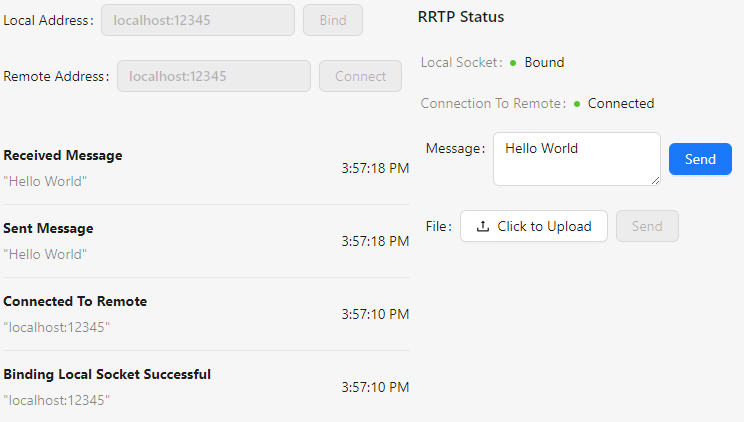
\includegraphics[width=\textwidth]{doc/latex/src/images/RRTP.png}
        \caption{Demo-ohjelman käyttöliittymä}
        \label{fig:demo_interface}
    \end{figure}
    
    Demo-ohjelmasta löytyy kaksi kenttää osoitteiden asettamiseen. Lista, joka
    pitää kirjaa tapahtumista. Tilannepaneeli, joka näyttää yhteyden tilan.
    Kaksi kenttää viestien ja tiedostojen lähettämiseen. \par

    \subsection{Riippuvuudet}
    Demo-sovelluksessa on mahdollista käyttää \textit{crates.io}-palvelun\footnote{Saatavilla osoitteesta: https://crates.io/} Rust-kirjastoja ja \textit{npm}-palvelun\footnote{Saatavilla osoitteesta: https://www.npmjs.com/} javascript-paketteja. Paketit mahdollistavat sovelluksen nopean kehityksen ja tarjoavat vakaita ratkaisuja eri ongelmiin. Usein pakettien käyttäminen on erittäin suositeltua, sillä niiden dokumentaatio ja valmiit ratkaisut ovat hyödyksi kehityksessä ja ylläpitämisessä.

    \begin{table}[h!]
        \centering
        \begin{tblr}{
            colspec = {lX},
        }
            Nimi               & Käyttötarkoitus                                               \\
            \hline
            tauri              & Käyttöliittymän piirtäminen                                   \\
            serde/bincode      & Tiedon serialisointi ja deserialisointi                       \\
            fern/log/humantime & Lokitiedostojen kirjoittaminen                                \\
            typeshare          & Typescript-rajapintojen luonti automaattisesti Rust-tyypeistä \\
            infer              & Tiedostotietojen lukeminen                                    \\
            thiserror/anyhow   & Virheilmoituksien luonti ja käsittely
        \end{tblr}
        \caption{Rust-riippuvuudet}
        \label{tab:cargo_dependencies}
    \end{table}


    \begin{table}[h!]
        \centering
        \begin{tblr}{
            colspec = {lll},
        }
            nimi            & käyttötarkoitus                           \\
            \hline
            ahooks          & hyödyllisiä react-koukkuja                \\
            antd            & käyttöliittymäelementit                  \\
            dayjs           & aikatietojen käsittely                   \\
            pretty-bytes    & tiedostokoon muuntaminen ihmisluettavaksi \\
            rc-virtual-list & virtuaaliset listat                       \\
            react/react-dom & käyttöliittymän hallinta ja piirtäminen   \\
            recoil          & käyttöliittymän tilan hallinta            \\
            typescript      & tyyppitietojen lisääminen javascriptiin   \\
            vite            & front-end ohjelmiston prosessointi
        \end{tblr}
        \caption{npm-riippuvuudet}
        \label{tab:npm_dependencies}
    \end{table}


    \subsection{Ohjelman käynnistysvaihe}

    Demo-ohjelma alkaa \lstinline{main.rs}-tiedoston \lstinline{fn main()}-funktiosta.
    Se suorittaa 5 tärkeää toimintoa: lokitus
    konfiguraatio, sovellustilan alustaminen, lokiseurantasäikeen käynnistys, IPC-rajapintojen määritys ja lopuksi käyttöliittymän käynnistys. \\



    Lokitus konfiguraatio tapahtuu \lstinline{setup_logger()}-funktion kautta, joka määrittelee lähdekoodin \ref{lst:logging_config} mukaiset asetukset.
    Lähdekoodissa \ref{lst:log_example} on havainnollistettu esimerkki lokitapahtumasta, josta ilmenee selkeästi tapahtuma aika,
    viestin taso, tapahtuman moduuli ja itse viestin sisältö.

    \begin{lstlisting}[caption={Esimerkki lokitapahtumasta}, label={lst:log_example}]
[2024-03-29T13:57:18Z INFO messanger::connection_processor]
Processing connection event:
ReceivedCompleteMessage([0, 72, 101, 108, 108, 111,
32, 87, 111, 114, 108, 100])
    \end{lstlisting}
    
    Lähdekoodi \ref{lst:log_example} esittää mahdollisen lokitapahtuman. Sovellus voi kirjoittaa lokitapahtuman käyttämällä \lstinline{log}-kirjaston tarjoamia makroja\footnote{Mahdolliset makrot ovat: debug, error, info, log, trace, warn.}: \lstinline|info!("Processing connection event: {:?}", event);|\par

    \begin{lstlisting}[caption={Lokituskonfiguraatio}, label={lst:logging_config}]
fern::Dispatch::new()
.format(|out, message, record| {
    out.finish(format_args!(
        "[{} {} {}] {}",
        humantime::format_rfc3339_seconds(SystemTime::now()),
        record.level(),
        record.target(),
        message
    ))
})
.level(log::LevelFilter::Debug)
.chain(std::io::stdout())
.apply()?;
    \end{lstlisting}


    Sovellustila alustetaan \lstinline{tauri:app:Builder} struktuurin \lstinline{setup}-funktiolla, jonka tunniste on kuvattu lähdekoodissa \ref{lst:setup_signature}. Funktion tunniste sisältää tiedot sen vaatimuksista, joita täytyy noudattaa sen sisällä. Näistä vaatimuksista \lstinline{Send} on erityisen tärkeä, sillä se takaa muistiturvallisuuden säikeiden välillä. Tämä mahdollistaa kanavien käytön sulkeumassa ilman muistiongelmia \cite[ch. 8.2]{rust-book}. \par

    \begin{lstlisting}[caption={Setup-funktion tunniste}, label={lst:setup_signature}]
pub fn setup<F>(mut self, setup: F) -> Self
where
F: FnOnce(&mut App<R>) ->
Result<(), Box<dyn std::error::Error>> + Send + 'static
    \end{lstlisting}


    \lstinline{setup} sulkeumassa, joka on kuvattu lähdekoodissa \ref{lst:setup}, luodaan lokituskanava riveillä 1\textendash4. Nämä kanavat mahdollistavat viestimisen säikeiden välillä ilman lukkoja. Tätä kanavaa pitkin Rust-prosessi pystyy lähettämään käyttöliittymään viestejä mistä tahansa säikeestä. Kanavan viestejä pystyy vastaanottamaan vain yhdessä paikassa\footnote{On olemassa Rust-yhteisön ylläpitämiä paketteja, jotka sallivat usean vastaanottajan, kuten \lstinline{crossbeam}.}, mutta viestien lähetyksessä ei ole tätä rajoitusta \cite[ch. 16.2]{rust-book}. Rivillä 7 luodaan säie viestien lukemista varten. Säie odottaa viestejä kanavasta ja saatuaan viestin, se välittää sen käyttöliittymään IPC-viestillä. Rivillä 5 luodaan sovelluksen tilarakenne, joka vastaanottaa lokikanavan lähettävän pään. Tämän jälkeen kutsutaan Tauri-sovelluskehystä hallitsemaan tätä tilaa.
    
    \begin{lstlisting}[caption={setup-sulkeuma}, label={lst:setup}]
let (log_sender, log_receiver): (
    Sender<LogSuccessMessage>,
    Receiver<LogSuccessMessage>,
) = std::sync::mpsc::channel();
let app_state = AppState::new(log_sender);
let handle = app.handle();
tauri::async_runtime::spawn(async move {
    loop {
        let message = log_receiver.recv().unwrap();
        match handle.emit_all("log", message) {
            Ok(_) => {}
            Err(e) => error!("Failed to emit log message: {}", e),
        }
    }
});
app.manage(app_state);\end{lstlisting}

    Sovelluksen tila sisältää yhteyden tilan, viestien tilan ja viitteen lokikanavan lähettävään päähän. Lähdekoodin \ref{lst:app_state} riveillä 11 ja 13 on huomattava, että nämä ovat \lstinline{Mutex<...>} primitiivin sisällä. \lstinline{ConnectorState} ja \lstinline{MessageState} eivät toteuta \lstinline{Send}-ominaisuutta, joka löytyy \lstinline{setup}-funktion tunnisteesta. \lstinline{Sender<...>} toteuttaa \lstinline{Send}-ominaisuuden, joten sitä ei tarvitse erikseen laittaa \lstinline{Mutex<...>}:in sisälle.

    
    \begin{lstlisting}[caption={Sovelluksen tilan rakenne}, label={lst:app_state}]
struct ConnectorState {
    pub connector: Option<ConnectionManager>,
    message_sender: Option<SyncSender<Vec<u8>>>,
}
#[derive(Default)]
struct MessageState {
    pub outgoing_file: Option<FileInfo>,
    pub incoming_file: Option<FileInfo>,
}
struct AppState {
    pub connector_state: Mutex<ConnectorState>,
    pub log_sender: Sender<LogSuccessMessage>,
    pub message_state: Arc<Mutex<MessageState>>,
}\end{lstlisting}

    \subsection{Prosessien välinen kommunikaatio}
    Tauri-sovelluskehys hyödyntää IPC-viestejä käyttöliittymän ja Rust-prosessin väliseen kommunikointiin.

    Tauri-sovelluskehys sisältää kaksi IPC-primitiiviä: tapahtumat ja komennot.
    Tapahtuma on yksisuuntainen viesti, joita käytetään pääosin ohjelmatilan muutoksien kommunikointiin. Lähdekoodissa \ref{lst:setup} rivillä 10 lähetetään tapahtuma, minkä käyttöliittymä vastaanottaa. Komento on Web API:n kaltainen viestintämenetelmä, jossa tieto siirtyy \textit{JSON-RPC} -kaltaisella protokollalla. Tämä mahdollistaa monimutkaisien tietorakenteiden käytön viestinnässä, sillä ne serialisoidaan JSON muotoon \cite{tauri-app}.

    \subsection{IPC-Komennot}
    IPC-komennot merkitään \lstinline{#[tauri::command]} attribuutilla. Funktio täytyy olla merkitty kyseillä attribuutilla, jotta sitä pystyy käyttämään lähdekoodin \ref{lst:ipc_commands} määrityksessä. Tauri pystyy tarjoamaan viitteet muun muassa sovellustilaan ja sovelluskahvaan käyttämällä \textit{Dependency Injection} nimistä suunnittelutapaa. Tämä suunnittelutapa on todella yleinen useissa sovelluskehyksissä kuten esimerkiksi ASP.NET Core:ssa \cite{DI_dotnet}. Tämä suunnittelutapa ei kuitenkaan ole yleinen Rust-kielessä, sillä se vaatii funktioden suorittamista dynaamisilla kutsuilla.
    ASP.NET Core:ssa \lstinline{Reflection} toiminnallisuus tarjoaa dynaamisen kutsumisen, joka tekee tästä suunnittelutavasta käytännöllisen.
    Tauri-sovelluskehys toteuttaa tämän täyttäen \lstinline{Procedural Macros} toimintoa. 


    Lähdekoodin \ref{lst:ipc_commands} määrittelee 5 IPC-komentoa, jota käytetään käyttöliittymän ja Rust-prosessin välisessä kommunikaatiossa. Näitä komentoja voidaan myöhemmin kutsua käyttöliittymästä käsin käyttäen \lstinline{invoke}-funktiota, kuten lähdekoodissa \ref{lst:calling_bind} on esitetty. \par

    \begin{lstlisting}[caption={IPC-komentojen määritys}, label={lst:ipc_commands}]
.invoke_handler(tauri::generate_handler![
    bind,
    connect,
    send_message,
    send_file_info,
    respond_to_file_info
])\end{lstlisting}

    \begin{lstlisting}[caption={'bind'-komennon kutsuminen}, label={lst:calling_bind}]
invoke<LogSuccessMessage>("bind", {address: localAddress})
.then((result) => {
    setLog(result);
    setConnectionStatus((prev) => ({...prev, local: true}));
})
.catch((err: LogErrorMessage) => {
    setLog(err);
    setConnectionStatus((prev) => ({...prev, local: false}));
});\end{lstlisting}

    \lstinline{bind}-komento liittää verkkosovittimen \lstinline{address} parametrin osoitteeseen. Liittämisen hoitaa \lstinline{ConnectionManager} rakenne, joka käynnistää myös tarvittavat säikeet viestien ja kuittauksien vastaanottoa varten, sekä säikeen viestien lähettämisetä varten. Lopuksi \lstinline{bind}-komento käynnistää säikeen, joka kuuntelee \lstinline{ConnectionManager}:n tuottamia tapahtumia.
    \lstinline{bind}-komennossa käynnistetty säie ohjaa \lstinline{ConnectionManager}:n tuottamat tapahtumat \lstinline{ConnectionProcessor} rakenteeseen, joka lajittelee tapahtumat niiden tyypin mukaan ja suorittaa tarvittavan strategian tapahtuman käsittelyyn.\par




    \lstinline{connect}-komento ottaa vastaan osoitteen ja sovellustilan, joka tulee Tauri:n DI-järjestelmästä ja käynnistää yhteyden. Lähdekoodissa \ref{lst:connect} rivillä 4 yhteyden tila lukitaan.
    Tämä on \lstinline{Mutex<...>} rakenteen toiminto. \lstinline{lock()}-funktio lukistee \lstinline{state.connector_state} muuttujaan ja palauttaa \lstinline{MutexGuard<ConnectorState>} rakenteen. Tämä suoja sallii muutoksien tekemisen \lstinline{ConnectorState} rakenteeseen, vaikka viite ei normaalisti salli muutoksia. Tätä piirrettä kutsutaan nimeltä \textit{Interior Mutability}. Yhteystila on lukittuna niin kauan kun \lstinline{MutexGuard<ConnectorState>} on käytössä.\par

    \begin{lstlisting}[basicstyle=\small\ttfamily,caption={'connect'-komento}, label={lst:connect}]
#[tauri::command]
pub fn connect(address: &str, state: State<AppState>)
-> LogMessageResult {
let app_state_lock = state.connector_state.lock().unwrap();
let connector = &app_state_lock.connector;
let result = connector
.as_ref()
.ok_or(LogErrorMessage::LocalSocketNotBound)?
.connect(address);
result
.map(|_| LogSuccessMessage::ConnectedToRemote(address.to_string()))
.map_err(|e| LogErrorMessage::ConnectionError(e.to_string()))
}\end{lstlisting}

    \lstinline{send_message, send_file_info ja respond_to_file_info} lähettävät tietoja verkon yli. \lstinline{send_message} lähettää yksinkertaisen viestin vastaanottajalle.
    \lstinline{send_file_info} lähettää vastaanottajalle tiedoston metatiedot: tiedoston nimi, tiedoston \textit{MIME}-tyyppi ja koko tavuina. Näiden tietojen avulla vastaanottaja pystyy valmistautumaan tulevaan tiedostoon. Kuva \ref{fig:incoming_file} havainnollistaa, miltä tuleva tiedosto näyttää vastaanottajalle. Vastaanottaja pystyy kuvan \ref{fig:incoming_file} mukaisella ikkunalla valitsemaan mihin kansioon kyseinen tiedosto tullaan tallentamaan tai vaihtoehtoisesti hylkäämään tulevan tiedoston. Valinnan tekeminen laukaisee \lstinline{respond_to_file_info}-IPC-komennon, joka ilmoittaa lähettäjälle valinnasta.
    Mikäli valinta on myönteinen, lähettäjä alkaa välittömästi lähettämään tiedostoa verkon yli. Jos valinta on kielteinen, lähettäjä saa ilmoituksen hylätystä tiedostosta.

    \begin{figure}[h!]
        \centering
        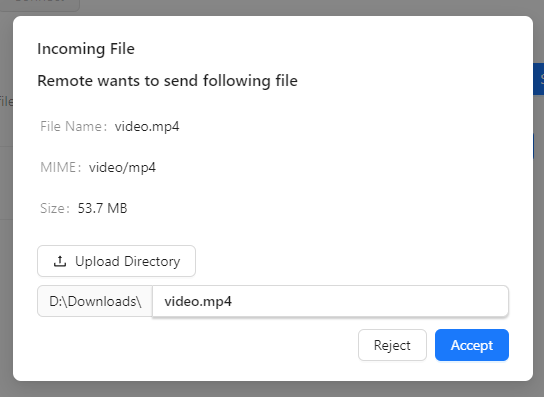
\includegraphics[width=0.5\textwidth]{doc/latex/src/images/incoming_file.png}
        \caption{Tulevan tiedoston tiedot}
        \label{fig:incoming_file}
    \end{figure}

    \section{Suorituskyky}\label{sec:suorityskyky}

    \subsection{Tietorakenteet}\label{sec:structures}
    Tämän ohjelman luonteen kannalta on tärkeää, että käytetään tehokkaita tietorakenteita. Ohjelman täytyy pystyä tehokkaasti käsittelemään listoja, jotka sisältävät tuhansia elementtejä. \par
    Mittauksessa mitattiin tavallisen taulukon, kasavaratun taulukon,
    \lstinline{Vec}:n, \lstinline{VecDeque} ja \lstinline{LinkedList} suoriutumista, kun tietorakenteen elementtejä siirretään vasemmalle. Jokainen tietorakenne täytettiin 100 000 elementillä ja elementtejä siirrettiin parhaiten sopivalla tavalla.
    Mittaus tehtiin käyttäen \textit{criterion}-kirjastoa ja 100:n näytemäärällä.

    Taulukon \ref{tab:collection_bench} tulosten perusteella kasataulukko on paras vaihtoehto mitatuista tietorakenteista. Tästä huolimatta projektissa käytettiin \lstinline{Vec} tietorakennetta, sillä taulukon koko ei ole tiedossa kääntämisen aikana.

    \begin{table}[h!]
        \centering
        \begin{tblr}{
            colspec = {ll},
        }
            Tietorakenne & Tulos     \\
            \hline
            Kasataulukko & 61.603 µs \\
            Taulukko     & 72.929 µs \\
            Vec          & 124.49 µs \\
            VecDeque     & 176.03 µs \\
            LinkedList   & 4.5944 ms \\
        \end{tblr}
        \caption{Tietorakenteiden nopeus elementtien siirrossa}
        \label{tab:collection_bench}
    \end{table}

    Tuloksista voidaan myös todeta, että \lstinline{LinkedList} tietorakennetta tulisi käyttää vain harvoissa tilanteissa. Rust-kielen standardikirjaston dokumentaatio vahvistaa tämän \cite{rust-linked-list}. Kääntäjä pystyy tekemään erinomaisia optimointeja näille muille tietorakenteille ja tietokoneen prosessori pystyy hyödyntämään välimuistia tehokkaammin.


    \subsection{Tiedostojen siirtäminen}


Tiedonsiirron testaamisessa käytettiin 30Mt kokoista videotiedostoa, jotta 
tiedoston eheys olisi mahdollisimman helppo tarkistaa.
Tässä testissä verrattiin RRTP-kirjaston, \textit{UDP}:n ja \textit{TCP}:n 
tiedonsiirtokykyä käyttäen silmukkaosoitetta. \par
Kuvasta \ref{fig:performance} voidaan päätellä, että 
RRTP-kirjaston suorituskyky on kohtalaisen hyvä verrattuna \textit{UDP}:hen ja \textit{TCP}:hen. \textit{TCP} on näistä selvästi nopein, mikä johtunee siitä, että
TCP:ssä puskurin käsittely on lähes automaattinen ja puskuri kasvaa tarvittaessa. 
\textit{UDP}:n ja RRTP-kirjaston kanssa käytettiin 128 tavun kokoista puskuria, mikä selittää näiden kahden tuloksen hitauden. Tulosten mukaan \textit{UDP} on 
hidas lähetyksen alussa mutta nopeutuu ajan kuluessa. Työn aikarajoitusten takia jatkotutkimusta tiedosiirron hitaudesta ei toteutettu. \par
    
    \begin{figure}[h!]
        \centering
        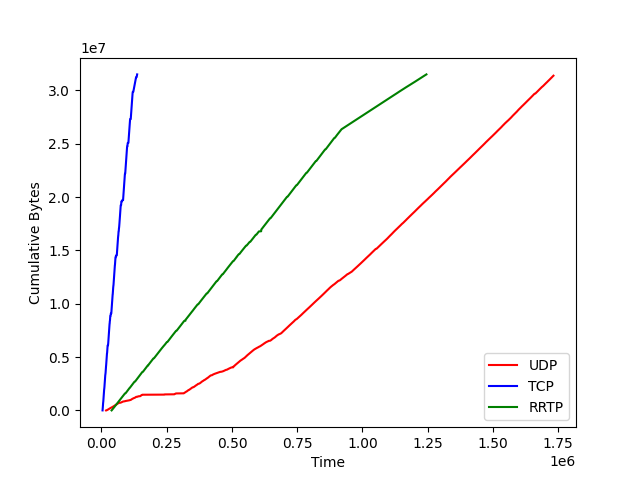
\includegraphics[width=\textwidth]{doc/latex/src/images/plot.png}
        \caption{Tiedonsiirtovertailun tulokset}
        \label{fig:performance}
    \end{figure}

    
Kokonaisuudessaan RRTP-kirjasto suoriutuu suhteellisen hyvin tehtävästään, mutta huomiota täytyy kiinnittää sen tehokkuuteen isoja tiedostoja siirrettäessä. Kuvasta \ref{fig:performance} nähdään, että kirjaston suorituskyky pienenee mitä enemmän tietoa on siirretty. Tämä johtunee siitä, että kirjaston sisäinen puskuri täytyy ja elementtien käsittely vie enemmän aikaa.



Silmukkaosoitteen takia tämä testi ei vastaa täysin todellisuutta.
Testin tarkoitus on pääasiassa seurata tietorakenteiden käsittelyn tehokkuutta ilman
verkon aiheuttamaa häiriötä.


    \section{Työkalut ja prosessit}
    Tässä työssä on käytetty alalla laajalti hyväksyttyjä sovelluskehitystapoja. Osa työkaluista ja menetelmistä on suhteellisen kokeellisia. Niitä käytettiin kuitenkin vain kehittäjäkokemuksen parantamiseen, eikä niitä käytetty työn kannalta kriittisissä osissa.

    \subsection{Versionhallinta}
    Tässä työssä käytettiin \textit{git}-versionhallintaa, \textit{github.com}-palvelun isännöimänä. Git on toimialalla erittäin yleinen ja tärkeä työkalu lähdekoodin jakamiseen ja versionhallintaan. \par

    \textit{Pull Request}:ien tekeminen on yleinen ja suositeltu tapa liittää muutokset pääharaan. Tämä johtuu siitä, että kun projektissa on useita ihmisiä tekemässä, jokainen muutos vaatii toisten kehittäjien hyväksynnän. Kun kriteerit hyväksymiseen on toteutunut,
    muutos liitetään päähaaraan.\par

    Työn toteutuksen aikana projektiin tuli noin 5 suurta refaktorointia.
    Näitä varten käytettiin useita haaroja, joiden avulla pystyttiin pitämään päähaara aina toimivassa tilassa. \par

    Projektin lähdekoodi on saatavilla \textit{github.com}-palvelusta osoitteesta:
    https://github.com/JoonasKajava/ReliableRealTimeTransportProtocol.

    \subsection{Kehitysympäristö}


    Alustana toimi taulukon \ref{tab:main_pc} pöytätietokone.
    Editorina pääsääntöisesti oli käytössä \textit{RustRover}\footnote{Saatavilla osoitteesta: https://www.jetbrains.com/rust/}, jossa oli muutama tärkeä lisäosa, kuten \textit{IdeaVim}, \textit{Grazie Pro}, \textit{SonarLint} ja \textit{WakaTime}.
    UDP-pakettien seurantaan käytin WireShark-ohjelmistoa.

    \begin{table}[h!]
        \centering
        \begin{tblr}{
            colspec = {ll},
        }
            Käyttöjärjestelmä & Microsoft Windows 10.0.19045 Pro    \\
            Rust-kääntäjä     & rustc 1.75.0 (82e1608df 2023-12-21) \\
            Node.js           & v18.8.0
        \end{tblr}
        \caption{Kehitysalustan tiedot}
        \label{tab:main_pc}
    \end{table}

    \section{Yhteenveto}
    Tavoitteena tässä opinnäytetyössä oli tutustua Rust-ohjelmointikieleen ja
    reaaliaikaisten kommunikaatiojärjestelmien luontiin. Työn tuloksena syntyi RRTP-kirjasto, joka hyödyntää liukuvaa ikkunaa ja muita toimintoja luotettavan yhteyden muodostamiseen.\par

    RRTP-kirjasto pystyy siirtämään viestejä ja tiedostoja ilman tiedon korruptiota. Lähdekoodi on suurimmaksi osaksi idiomaattista Rust-koodia ja käyttöliittymän React-koodi käyttää ajankohtaisia suosituksia ja menetelmiä.
    Koodi on jaettu yksinkertaisiin moduuleihin ja suunniteltu niin, että laajennukset tai muutokset ovat helppoja toteuttaa.\par

    Jatkokehityspolku on selkeä. Protokollaan voidaan toteuttaa lisää TCP:n hyödyntämiä tekniikoita, kuten dynaaminen aikakatkaisu paketeille ja dynaaminen koko liukuvalle ikkunalle. Nämä kaksi tekniikkaa saadaan helposti lisättyä, koska muutokset otettiin huomioon arkkitehtuurin suunnittelussa.\par

    Lopputuloksena syntyi vakaa ja toimiva kirjasto reaaliaikaiselle kommunikaatiolle. Kirjasto kirjoitettiin kokonaan käyttäen turvallista Rust-kieltä, joka 
    Rust takaa muistiturvallisuuden samalla tavalla kuin ohjelmointikielet, jotka käyttävät automaattista roskienkeräystä. Lisäksi Rust-kielen vaativa syntaksi ja
    tyyppimallit takaavat, että ohjelmassa ei voi olla epäkelpoisia tiloja.
    Tätä filosofiaa pystyttiin myös jatkamaan käyttöliittymän puolella käyttämällä
    tarkkoja TypeScript sääntöjä sekä TypeShare-kirjastoa, jotta Rust-tyypit saatiin vastaamaan täsmälleen TypeScript-tyyppejä.\par

    Protokollan kehityksessä tutustuttiin säikeiden turvalliseen käyttöön ja miten Rust-kieli auttaa tässä. Tärkeänä osana oli myös toteuttaa toimiva käyttöliittymä, joka pystyy hyödyntämään Rust-kielen vahvuuksia. Tämä on erityisen tärkeää sillä
    uskon vahvasti, että Rust-kieli on tulevaisuuden kieli. Sitä käytetään jo muun muassa Linux:n ja Windows:n kernelissä. Rust-kielen turvallisuus, tehokkuus ja modernit ominaisuudet tekevät siitä lähes täydellisen kielen, jolla on mahdollisuus korvata C ja C++ tulevaisuudessa.


    \newpage
    \printbibliography
\end{document}
